% Dit werk is gelicenseerd onder de licentie Creative Commons Naamsvermelding-GelijkDelen 4.0 Internationaal. Ga naar http://creativecommons.org/licenses/by-sa/4.0/ om een kopie van de licentie te kunnen lezen.
\documentclass[t]{beamer}

\usepackage{amsmath,amsthm}             % Uitgebreide wiskundige mogelijkheden
\usepackage{xcolor}						% Om kleuren te gebruiken

%%%%%%%%%%%%%%%%%%%%%%%%%%%%%%%%%%%%%%%%%%%%%%%%%%%%%%%%%%%%
% Nieuwe commandos
%%%%%%%%%%%%%%%%%%%%%%%%%%%%%%%%%%%%%%%%%%%%%%%%%%%%%%%%%%%%

% De differentiaal operator
\newcommand{\diff}{\ensuremath{\mathrm{d}}}
\newcommand{\subsdiff}{\ensuremath{\mathrm{D}}}
\newcommand{\vardiff}{\ensuremath{\mathrm{\delta}}}

% Super en subscript
\newcommand{\supsc}[1]{\ensuremath{^{\text{#1}}}}   % Superscript in tekst
\newcommand{\subsc}[1]{\ensuremath{_{\text{#1}}}}   % Subscript in tekst

% Vectoren en matrices
\newcommand{\vt}[1]{\ensuremath{\boldsymbol{#1}}} % vector in juiste lettertype
\newcommand{\mx}[1]{\ensuremath{\mathsf{#1}}}	  % matrix in juiste lettertype

% Nieuw commando om iets te benadrukken en tegelijkertijd in de index te steken.
\newcommand{\begrip}[1]{\index{#1}\textbf{#1}\xspace}

% Graden celcius
\newcommand{\degC}{\ensuremath{^\circ \mathrm{C}}}
% graden
\renewcommand{\deg}{\ensuremath{^\circ}}

% unit
\newcommand{\unit}[1]{\ensuremath{\mathrm {#1}}}


% underlinered
\newcommand{\underlinered}[1]{\color{red}\underline{{\color{black}#1}}\color{black}}
%%%%%%%%%%%%%%%%%%%%%%%%%%%%%%
% Packages
%%%%%%%%%%%%%%%%%%%%%%%%%%%%%%

%\usepackage{geometry}              	% 
\usepackage[dutch]{babel}               % Voor nederlandstalige hyphenatie (woordsplitsing)
\uselanguage{dutch}
\languagepath{dutch}
\usepackage{amsmath,amsthm}             % Uitgebreide wiskundige mogelijkheden
\usepackage{url}                        % Om url's te verwerken
\usepackage{graphicx,subfigure}         % Om figuren te kunnen verwerken
\usepackage[utf8]{inputenc}             % Om niet ascii karakters rechtstreeks te kunnen typen
\usepackage[section]{placeins}			% Om ervoor te zorgen dat floats binnen dezelfde section blijven
\usepackage{multicol}
\usepackage[absolute,overlay]{textpos}

%%%%%%%%%%%%%%%%%%%%%%%%%%%%%%
% Layout
%%%%%%%%%%%%%%%%%%%%%%%%%%%%%%
\usetheme{Frankfurt}
\usefonttheme[onlymath]{serif}
\AtBeginSection[]
{
  \begin{frame}
    \frametitle{Inhoud}
    \tableofcontents[currentsection]
  \end{frame}
}

\setbeamertemplate{navigation symbols}{}
\setbeamertemplate{footline}[page number]

%%%%%%%%%%%%%%%%%%%%%%%%%%%%%%
% Title
%%%%%%%%%%%%%%%%%%%%%%%%%%%%%%
\title{Fluïdummechanica}
\author{Brecht Baeten\inst{1}}
\institute{
	\inst{1}%
  		KU Leuven, Technologie campus Diepenbeek,\\ e-mail: brecht.baeten@kuleuven.be
}
\date{\today}
%%%%%%%%%%%%%%%%%%%%%%%%%%%%%%
% Omgevingen
%%%%%%%%%%%%%%%%%%%%%%%%%%%%%%


\subtitle{Vormweerstand en vleugelprofielen}

\begin{document}

	\frame{\titlepage}
%%%%%%%%%%%%%%%%%%%%%%%%%%%%%%%%%%%%%%%%%%%%%%%%%%%%%%%%%%%%%%%%%%%%%%%%%%%
	\section{Inleiding}
	\begin{frame}
		\frametitle{Voorbeeld}
		\center
		\vspace{-0.5cm}
    	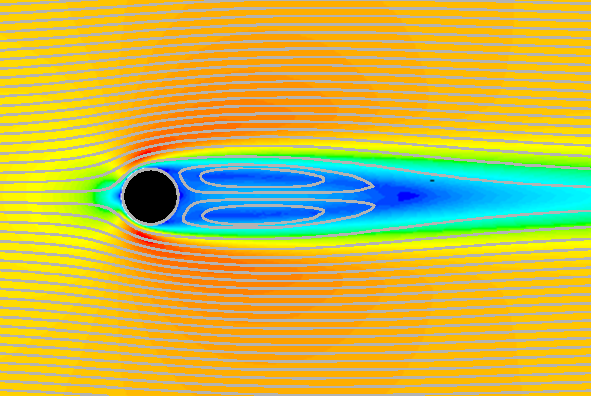
\includegraphics[width=\textwidth]{../fig/uitwendige_stroming/Cilinderstroming_snelheid_stroomlijnen_Re100}
  	\end{frame}
%%%%%%%%%%%%%%%%%%%%%%%%%%%%%%%%%%%%%%%%%%%%%%%%%%%%%%%%%%%%%%%%%%%%%%%%%%%
	\begin{frame}
		\frametitle{Weerstandscoëfficiënt}
		Op elk voorwerp in een stroming wordt een kracht in de richting van de stroming uitgeoefend.
		
		\pause
		\begin{center}
			Weerstandskracht
		\end{center}			
		
		\pause
		Dimensieanalyse:
		\begin{equation*}
    		F_\mathrm{d} = f\left( \rho,v,\nu,D,\mathrm{vorm} \right)
    	\end{equation*}
		
		\pause
		\vspace{0.3cm}
		\begin{center}
			Weerstandscoëfficiënt
		\end{center}
    	\begin{equation}
    		C_\mathrm{d} = \frac{F_\mathrm{d}}{1/2 \rho v^2 A}
    	\end{equation}
    	\begin{equation*}
    		C_\mathrm{d}(\mathrm{Re},\mathrm{vorm})
    	\end{equation*}
  	\end{frame}
%%%%%%%%%%%%%%%%%%%%%%%%%%%%%%%%%%%%%%%%%%%%%%%%%%%%%%%%%%%%%%%%%%%%%%%%%%%
  	\begin{frame}
		\frametitle{Demo}
		\center
    	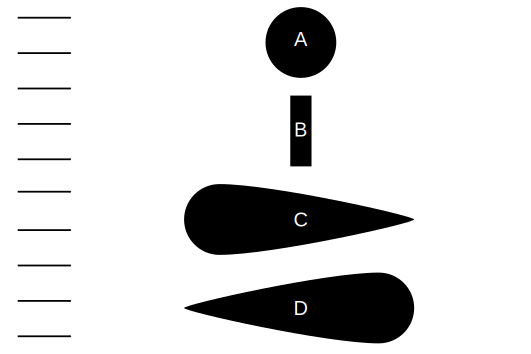
\includegraphics[height=0.8\textheight]{../fig/uitwendige_stroming/Invloed_van_vorm_op_weerstand}
  	\end{frame}
%%%%%%%%%%%%%%%%%%%%%%%%%%%%%%%%%%%%%%%%%%%%%%%%%%%%%%%%%%%%%%%%%%%%%%%%%%%
	\section{Potentiaalstroming}
	\begin{frame}
		\frametitle{Potentiaalstroming}
		\only<1-2>{
			Euler vergelijkingen voor 2D stationaire stroming
			\begin{align*}
				\rho v_x \frac{\partial v_x}{\partial x} + \rho v_y \frac{\partial v_x}{\partial y} &= -\frac{\partial p}{\partial x} + g_x \\
				\rho v_x \frac{\partial v_y}{\partial x} + \rho v_y \frac{\partial v_y}{\partial y} &= -\frac{\partial p}{\partial y} + g_y \\
				\frac{\partial v_x}{\partial x} + \frac{\partial v_y}{\partial y} = 0
			\end{align*}
		}
		\only<2>{
			Rotatie is constant
		}
		\only<2-5>{
			\begin{equation*}
				\omega = \frac{\partial v_y}{\partial x} - \frac{\partial v_x}{\partial y} = \mathrm{Cst}
			\end{equation*}
		}
		\only<4-5>{
			Indien de rotatie nul is ($\omega=0$):\\
			\vspace{0.5cm}
		}
		\only<5-5>{
			Er bestaat een stroom- en potentiaalfunctie die voldoet aan de Laplace vergelijking waaruit de snelheidscomponenten kunnen afgeleid worden.
			\begin{equation}
			\frac{\partial^2 \psi}{\partial x^2} + \frac{\partial^2 \psi}{\partial y^2} = 0
			\end{equation}
			\begin{align}
				v_x &=  \frac{\partial \psi}{\partial y} \\
				v_y &= -\frac{\partial \psi}{\partial x}
			\end{align}
		}
  	\end{frame}
%%%%%%%%%%%%%%%%%%%%%%%%%%%%%%%%%%%%%%%%%%%%%%%%%%%%%%%%%%%%%%%%%%%%%%%%%%%
	\begin{frame}
		\frametitle{Stroomfunctie}
		
		\center
		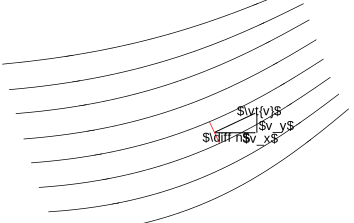
\includegraphics{../fig/uitwendige_stroming/Stroomfunctie}
			
  	\end{frame}
%%%%%%%%%%%%%%%%%%%%%%%%%%%%%%%%%%%%%%%%%%%%%%%%%%%%%%%%%%%%%%%%%%%%%%%%%%%
	\section{Stroming rond een cilinder}
  	\begin{frame}
		\frametitle{Potentiaalstroming}
		\only<1>{
			\begin{itemize}
				\item Poolcoördinaten
				\item Randvoorwaarden, ver van de cilinder en op de cilinderwand
				\item Superpositie van uniforme stroming en doublet
			\end{itemize}
		}
		\only<2>{
			\center
			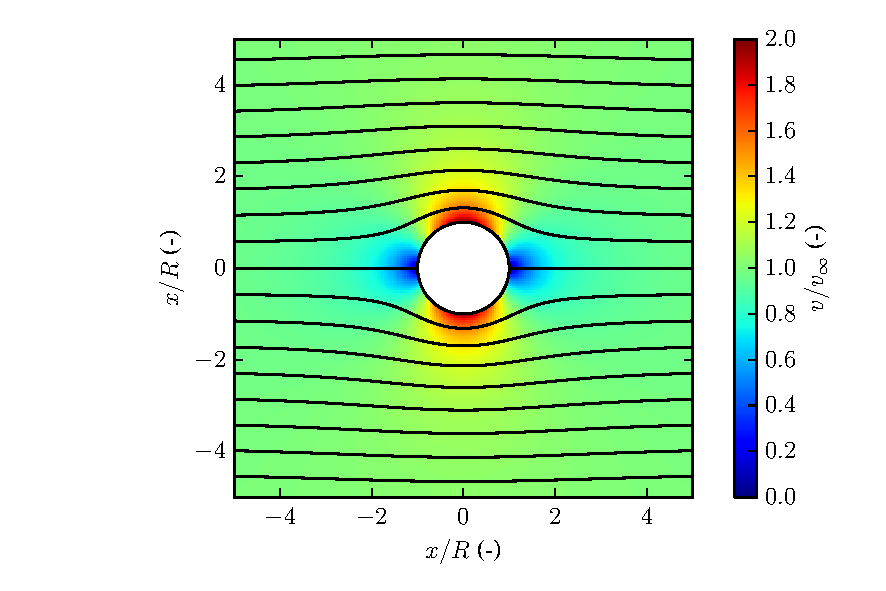
\includegraphics[height=0.8\textheight]{../fig/uitwendige_stroming/Potentiaalstroming_cilinder_snelheid}
		}
		\only<3>{
			\center
			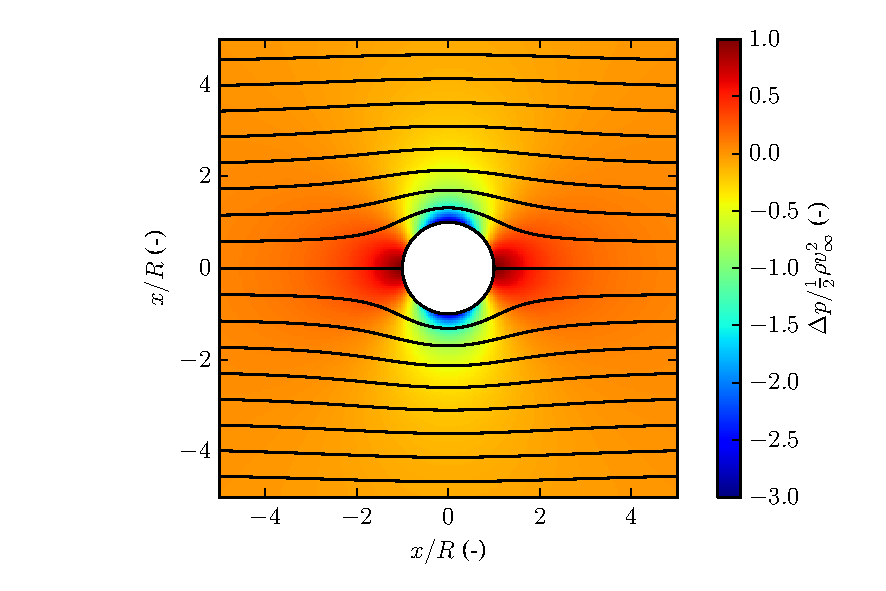
\includegraphics[height=0.8\textheight]{../fig/uitwendige_stroming/Potentiaalstroming_cilinder_druk}
		}
		\only<4>{
			\center
			\vfill
			Potentiaalstroming rond een cilinder geeft geen weerstandskracht
			\vfill
		}
  	\end{frame}
%%%%%%%%%%%%%%%%%%%%%%%%%%%%%%%%%%%%%%%%%%%%%%%%%%%%%%%%%%%%%%%%%%%%%%%%%%%	
  	\begin{frame}
		\frametitle{Kruipende stroming}
		\only<1-2>{
			\begin{itemize}
				\item Zeer lage snelheid
				\item Zeer hoge viskeuze krachten
				\item Gekarakteriseerd door een zeer laag Reynoldsgetal
			\end{itemize}
		}
		\only<2>{
			\vspace{1cm}
			\center
			Analytische oplossing mogelijk\\ Stokes flow
		}
		\only<3-5>{
			\begin{textblock}{5}(13,3)
           		$\mathrm{Re}=1$
        	\end{textblock}
		}
		\only<3>{
			\hspace{1.2cm}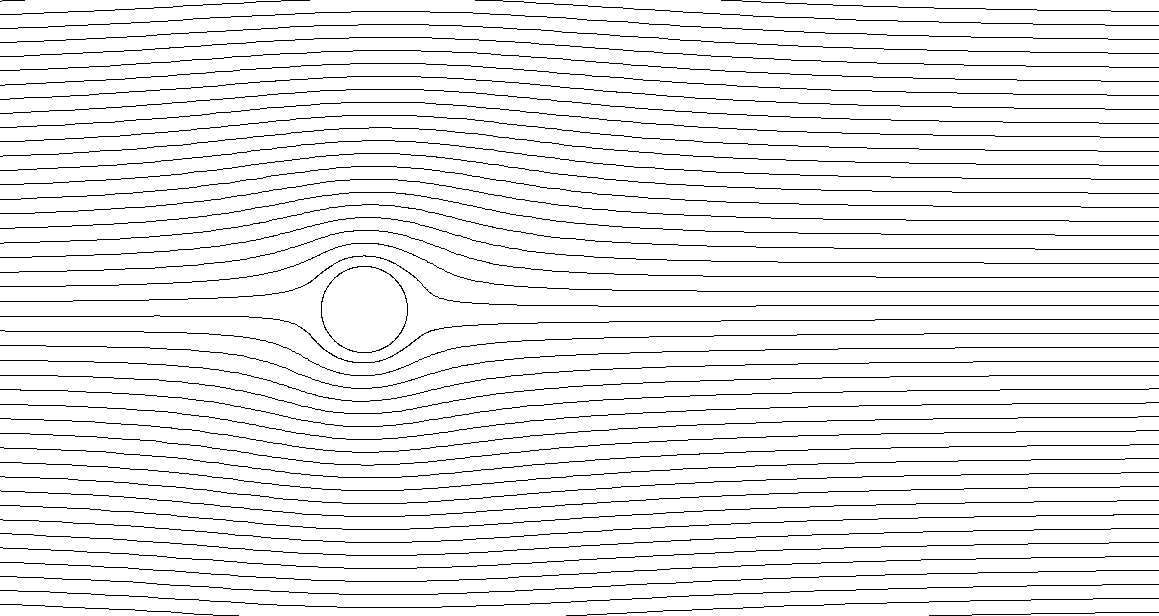
\includegraphics[height=0.40\textheight]{../fig/uitwendige_stroming/Stroomfunctie_Re1_bw}
			\vspace{0.1cm}
			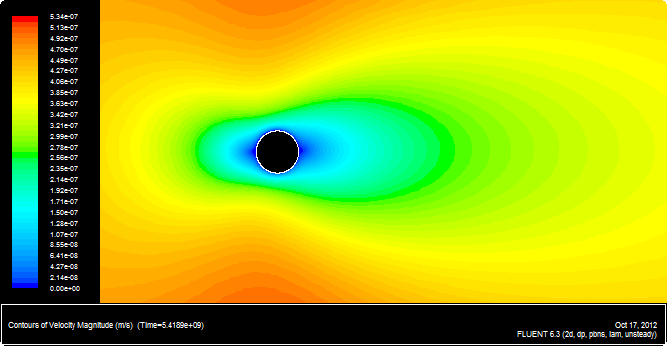
\includegraphics[height=0.47\textheight]{../fig/uitwendige_stroming/Cilinderstroming_snelheid_Re1}
		}
		\only<4>{
			\vspace{0.3cm}
			\center
			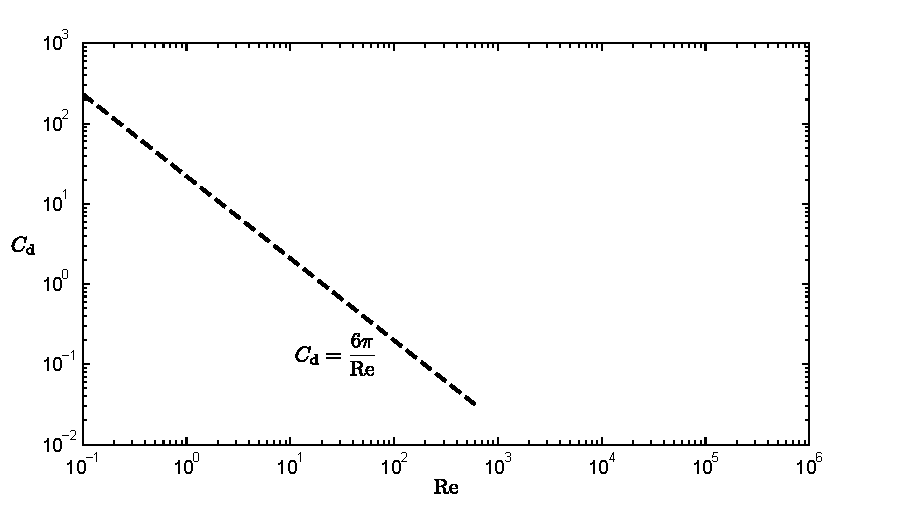
\includegraphics[width=\textwidth]{../fig/uitwendige_stroming/Cilinderstroming_Cd_kruipend}
		}
		\only<5>{
			\vspace{0.3cm}
			\center
			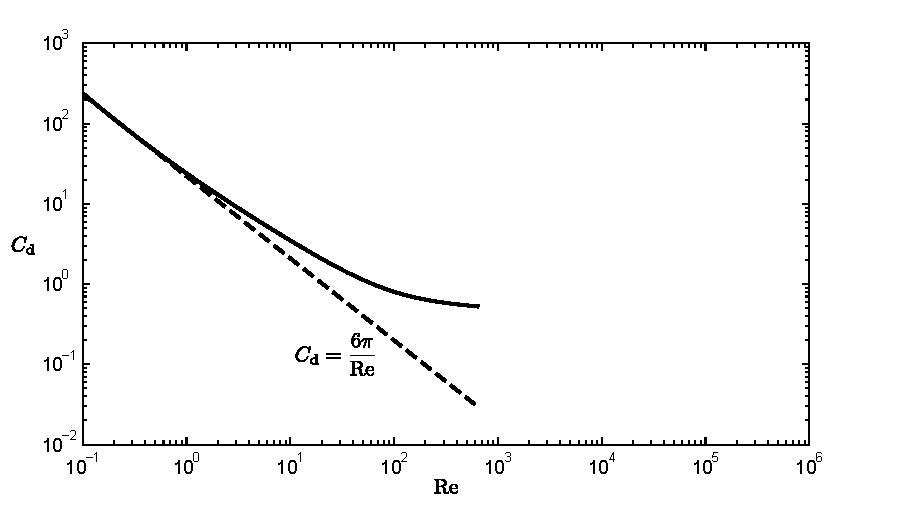
\includegraphics[width=\textwidth]{../fig/uitwendige_stroming/Cilinderstroming_Cd_kruipend_werkelijk}
		}
  	\end{frame}
%%%%%%%%%%%%%%%%%%%%%%%%%%%%%%%%%%%%%%%%%%%%%%%%%%%%%%%%%%%%%%%%%%%%%%%%%%%
  	\begin{frame}
		\frametitle{Viskeuze stroming}
		\only<1>{
			\begin{textblock}{5}(13,3)
           		$\mathrm{Re}=10$
        	\end{textblock}
			\hspace{1.2cm}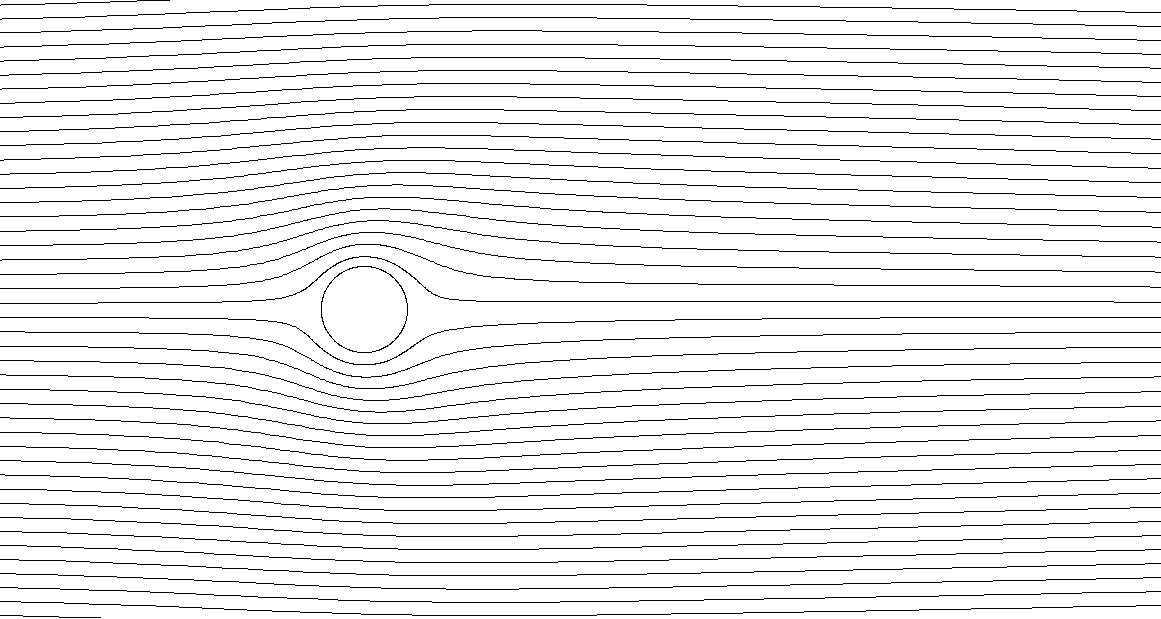
\includegraphics[height=0.40\textheight]{../fig/uitwendige_stroming/Stroomfunctie_Re10_bw}
			\vspace{0.1cm}
			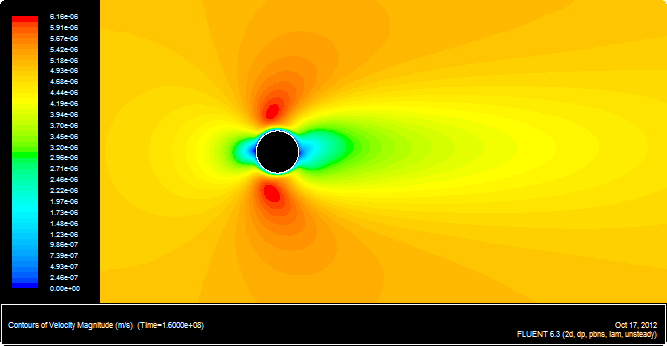
\includegraphics[height=0.47\textheight]{../fig/uitwendige_stroming/Cilinderstroming_snelheid_Re10}
		}
		\only<2>{
			\begin{textblock}{5}(13,3)
           		$\mathrm{Re}=100$
        	\end{textblock}
			\hspace{1.2cm}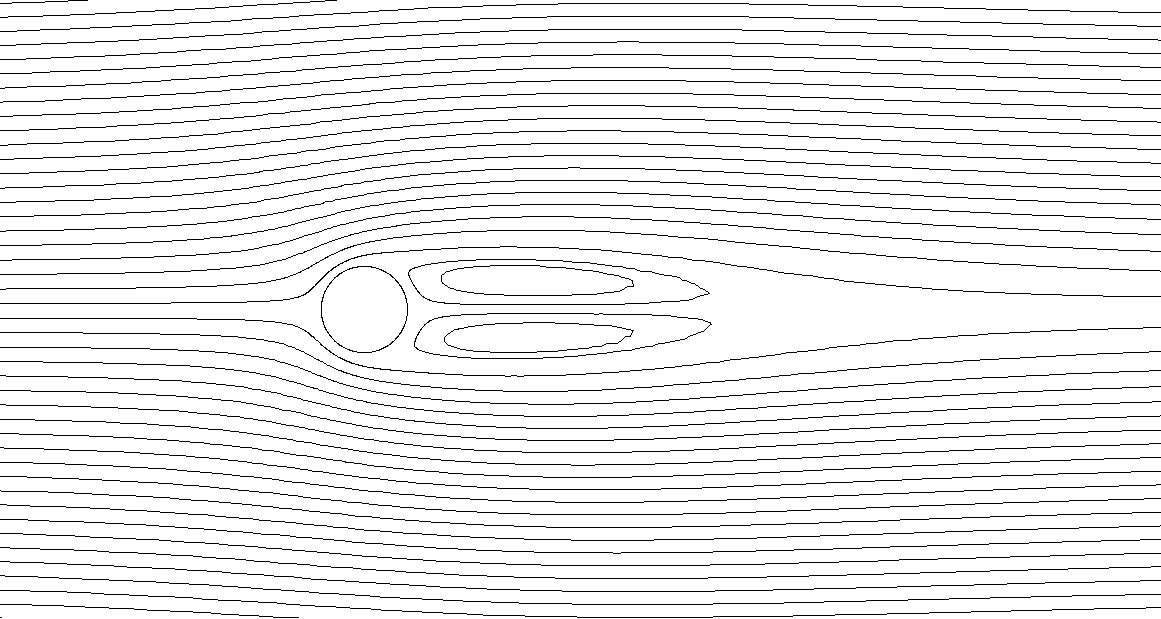
\includegraphics[height=0.40\textheight]{../fig/uitwendige_stroming/Stroomfunctie_Re100_bw}
			\vspace{0.1cm}
			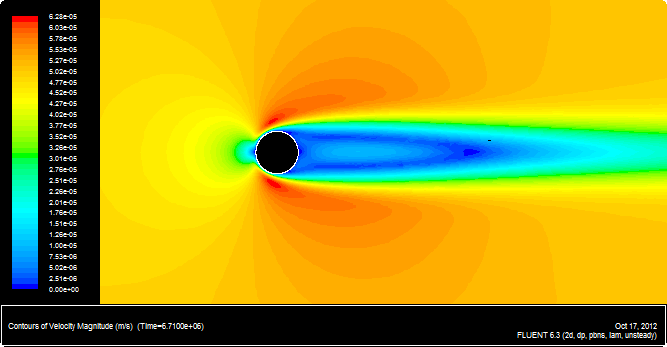
\includegraphics[height=0.47\textheight]{../fig/uitwendige_stroming/Cilinderstroming_snelheid_Re100}
		}
		\only<3>{
			\begin{textblock}{5}(13,3)
           		$\mathrm{Re}=250$
        	\end{textblock}
        	\center
        	\vspace{1cm}
			\href{run:fig/uitwendige_stroming/Von_Karman_vortex_street_laminar_temperature_Re250.mp4}{
				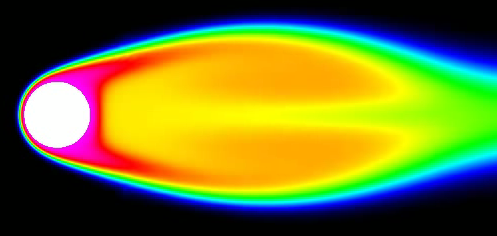
\includegraphics[width=0.8\textwidth]{../fig/uitwendige_stroming/Von_Karman_vortex_street_laminar_temperature_Re250.png}
			}\\
			\footnotesize{Bron: https://www.youtube.com/watch?v=IDeGDFZSYo8}
		}
		\only<4>{
			\begin{textblock}{5}(13,3)
           		$\mathrm{Re}=1 000$
        	\end{textblock}
			\hspace{1.2cm}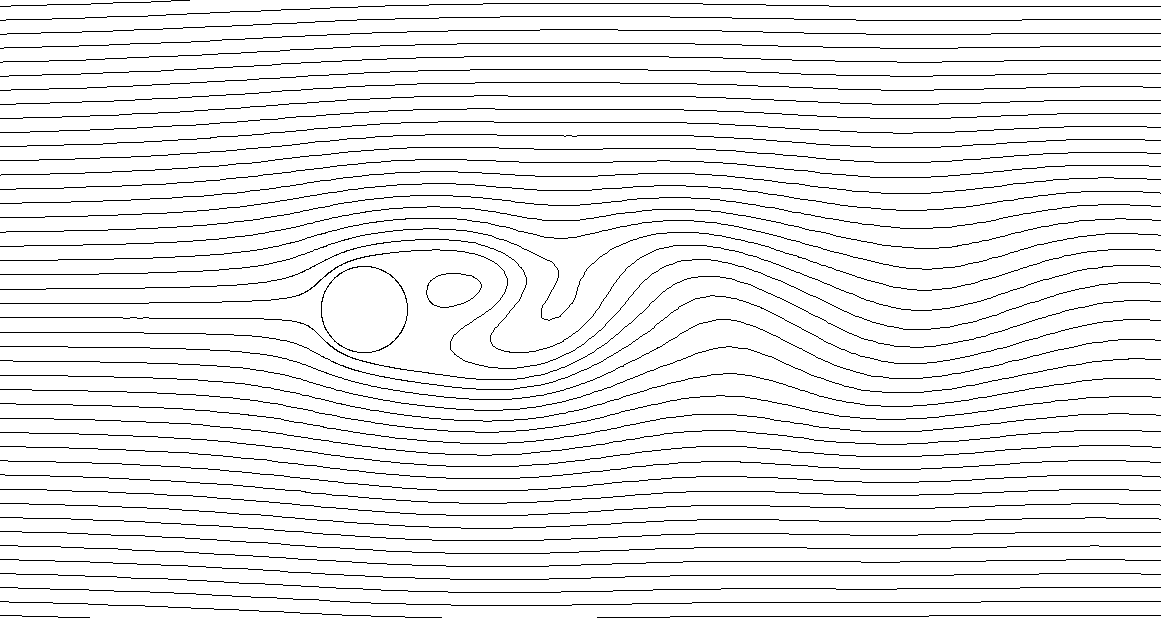
\includegraphics[height=0.40\textheight]{../fig/uitwendige_stroming/Stroomfunctie_Re1000_bw}
			\vspace{0.1cm}
			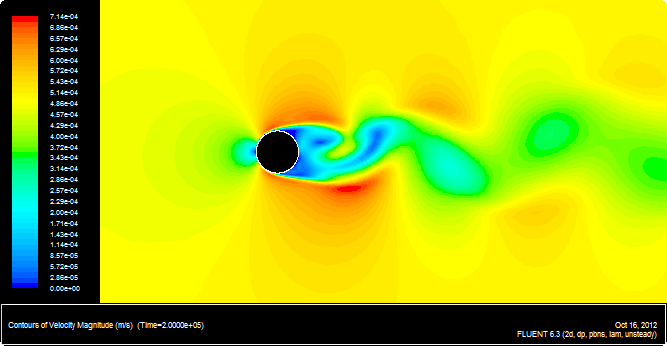
\includegraphics[height=0.47\textheight]{../fig/uitwendige_stroming/Cilinderstroming_snelheid_Re1000}
		}
		\only<5>{
			\begin{textblock}{5}(13,3)
           		$\mathrm{Re}=100 000$
        	\end{textblock}
        	% deze afbeelding is eigenlijk met Re=10000 maar het verloop is gelijkaardig
			% geen tijd om een nieuwe afbeelding te maken 
			\hspace{1.2cm}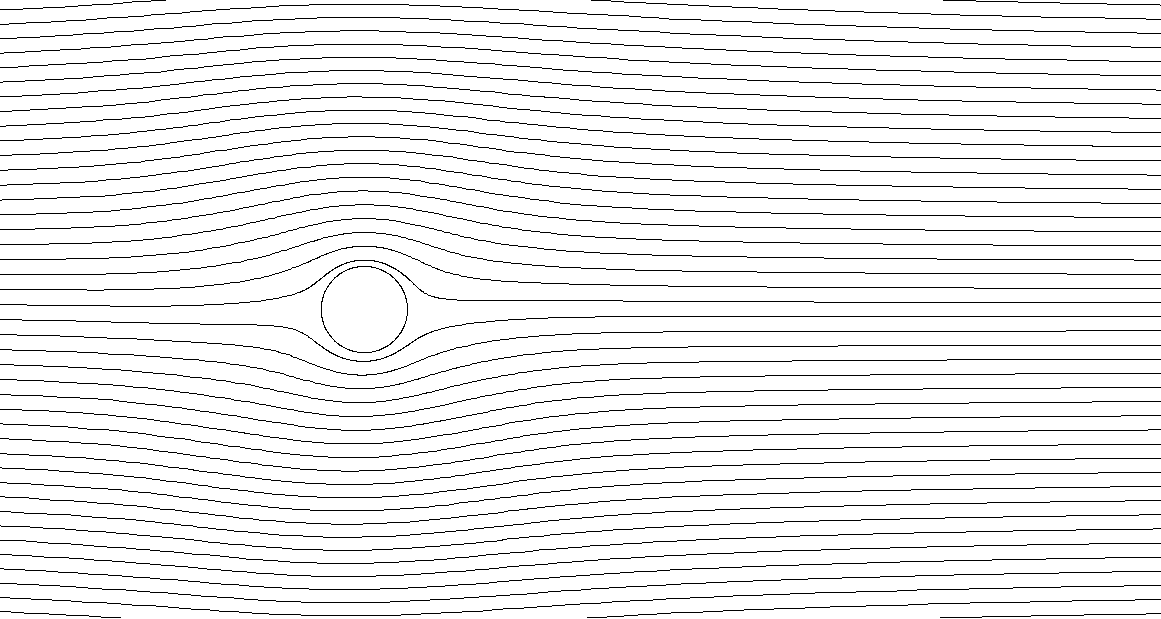
\includegraphics[height=0.40\textheight]{../fig/uitwendige_stroming/Stroomfunctie_Re10000_bw}
			\vspace{0.1cm}
			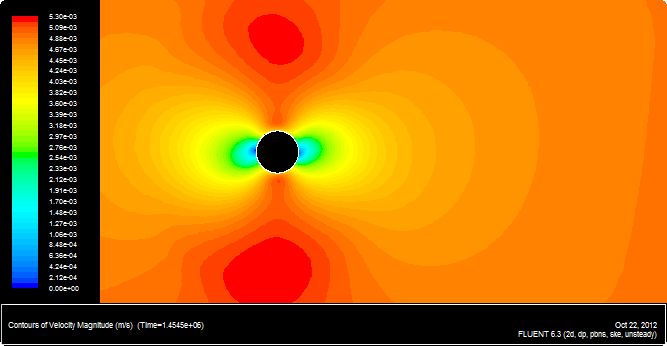
\includegraphics[height=0.47\textheight]{../fig/uitwendige_stroming/Cilinderstroming_snelheid_Re10000}
		}
  	\end{frame}
%%%%%%%%%%%%%%%%%%%%%%%%%%%%%%%%%%%%%%%%%%%%%%%%%%%%%%%%%%%%%%%%%%%%%%%%%%%
  	\begin{frame}
  		\frametitle{Weerstandscoëfficiënt}
  		\center
  		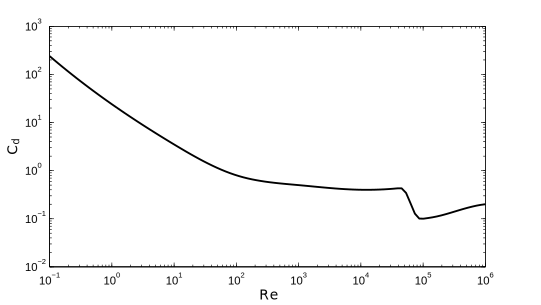
\includegraphics[width=\textwidth]{../fig/uitwendige_stroming/Cilinderstroming_Cd}
  	\end{frame}
%%%%%%%%%%%%%%%%%%%%%%%%%%%%%%%%%%%%%%%%%%%%%%%%%%%%%%%%%%%%%%%%%%%%%%%%%%%
	\section{Loshechting}
	\begin{frame}
		\frametitle{Drukverloop}
		\pause
		\center
		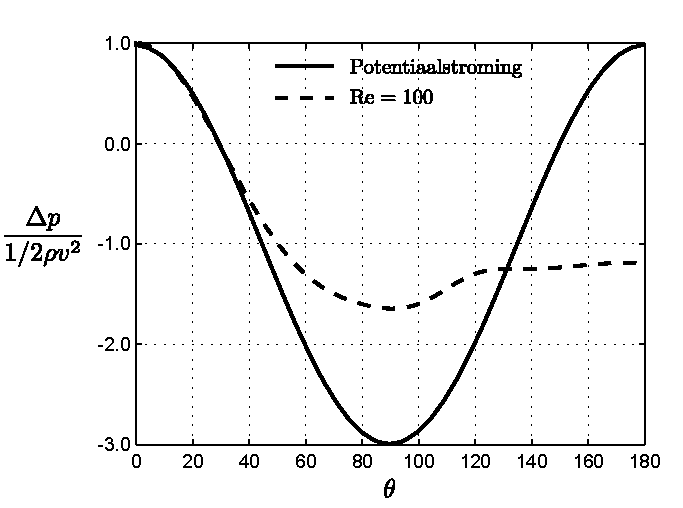
\includegraphics[width=0.8\textwidth]{../fig/uitwendige_stroming/Cilinderstroming_drukverloop}
  	\end{frame}
%%%%%%%%%%%%%%%%%%%%%%%%%%%%%%%%%%%%%%%%%%%%%%%%%%%%%%%%%%%%%%%%%%%%%%%%%%%	
  	\begin{frame}
		\frametitle{Loshechting}
		\pause
		\center
		\includegraphics{../fig/uitwendige_stroming/loshechting}
  	\end{frame}
%%%%%%%%%%%%%%%%%%%%%%%%%%%%%%%%%%%%%%%%%%%%%%%%%%%%%%%%%%%%%%%%%%%%%%%%%%%	
  	\begin{frame}
		\frametitle{Loshechting}
		Voorzijde:
		\begin{center}
			Druk wordt omgezet naar kinetische energie
		\end{center}
		
		\vspace{0.5cm}
		\pause
		Achterzijde:
		\begin{center}
			Kinetische energie moet terug worden omgezet in drukstijging
			
			\vspace{0.5cm}
			\pause
			Energie is gedeeltelijk gedissipeerd door viskeuze wrijving
			
			\vspace{0.5cm}
			\pause
			Achterste stagnatiepunt verschuift en de druk wordt niet verder opgebouwd
		\end{center}
  	\end{frame}
%%%%%%%%%%%%%%%%%%%%%%%%%%%%%%%%%%%%%%%%%%%%%%%%%%%%%%%%%%%%%%%%%%%%%%%%%%%
  	\begin{frame}
  		\frametitle{Weerstandscoëfficiënt}
  		\center
  		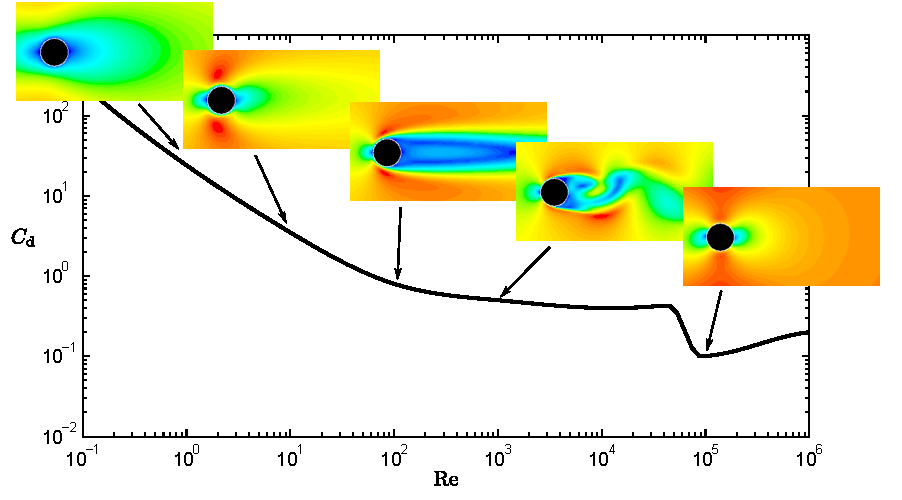
\includegraphics[width=\textwidth]{../fig/uitwendige_stroming/Cilinderstroming_Cd_snelheidsvelden}
  	\end{frame}
%%%%%%%%%%%%%%%%%%%%%%%%%%%%%%%%%%%%%%%%%%%%%%%%%%%%%%%%%%%%%%%%%%%%%%%%%%%
  	\begin{frame}
		\frametitle{Demo}
		\center
    	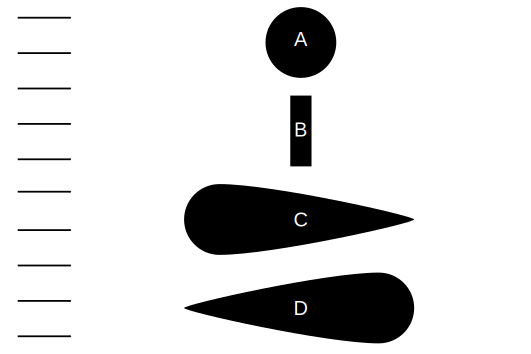
\includegraphics[height=0.8\textheight]{../fig/uitwendige_stroming/Invloed_van_vorm_op_weerstand}
  	\end{frame}
%%%%%%%%%%%%%%%%%%%%%%%%%%%%%%%%%%%%%%%%%%%%%%%%%%%%%%%%%%%%%%%%%%%%%%%%%%%
  	\begin{frame}
		\frametitle{Oppervlakte weerstand - Vorm weerstand}
		\center
    	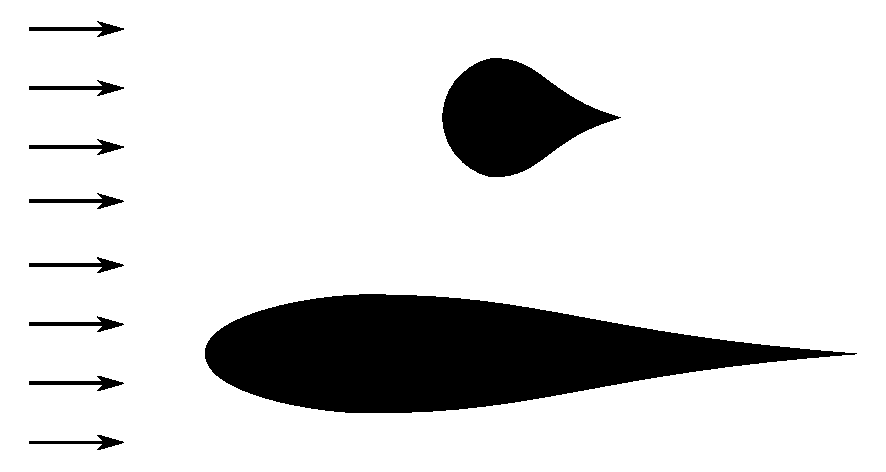
\includegraphics[width=\textwidth]{../fig/uitwendige_stroming/Vormweerstand-oppervlakteweerstand}
  	\end{frame}
%%%%%%%%%%%%%%%%%%%%%%%%%%%%%%%%%%%%%%%%%%%%%%%%%%%%%%%%%%%%%%%%%%%%%%%%%%%
	\section{Vleugelprofielen}
	\begin{frame}
		\frametitle{Definities}
		\only<1>{
			\vspace{0.5cm}
			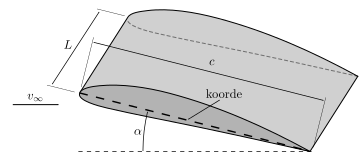
\includegraphics[width=\textwidth]{../fig/uitwendige_stroming/Vleugelprofiel_3D}
		}
		\only<2>{
			\vspace{0.5cm}
			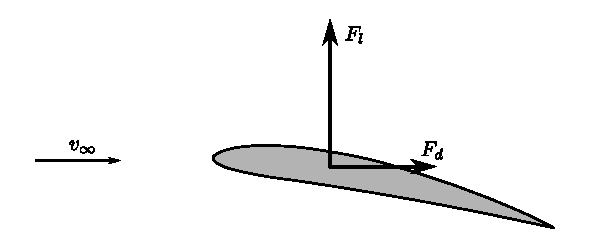
\includegraphics[width=\textwidth]{../fig/uitwendige_stroming/Vleugelprofiel_krachten}
		}
		\only<3-4>{
			\vspace{-0.5cm}
			\begin{center}
				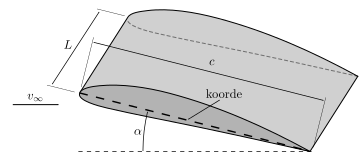
\includegraphics[width=3cm]{../fig/uitwendige_stroming/Vleugelprofiel_3D} \hspace{1.5cm}
           		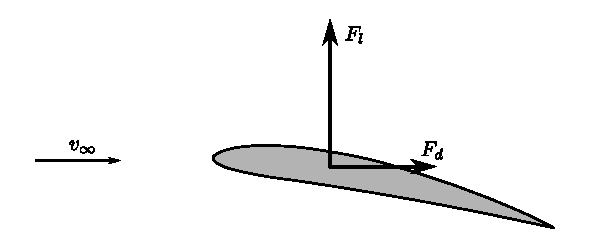
\includegraphics[width=3cm]{../fig/uitwendige_stroming/Vleugelprofiel_krachten}
			\end{center}
           	
           	\vspace{-0.3cm}
           	Dimensieanalyse:
           	\vspace{-0.3cm}
			\begin{align*}
				F_\mathrm{d} &= f\left( \rho,v,\nu,c,L,\alpha,\mathrm{vorm} \right)\\
    			F_\mathrm{l} &= g\left( \rho,v,\nu,c,L,\alpha,\mathrm{vorm} \right)
    		\end{align*}
		}
		\only<4-4>{
			\vspace{-0.5cm}
			\begin{center}
				Weerstands- en Liftcoëfficiënt
			\end{center}
			\vspace{-0.3cm}
    		\begin{align}
    			C_\mathrm{d} &= \frac{F_\mathrm{d}}{1/2 \rho v^2 A}\\
    			C_\mathrm{l} &= \frac{F_\mathrm{l}}{1/2 \rho v^2 A}
    		\end{align}
    		\begin{equation*}
    			A= c L \qquad C_\mathrm{d}(\alpha,\mathrm{Re},\mathrm{vorm}) \qquad C_\mathrm{l}(\alpha,\mathrm{Re},\mathrm{vorm})
    		\end{equation*}
		}
  	\end{frame}
%%%%%%%%%%%%%%%%%%%%%%%%%%%%%%%%%%%%%%%%%%%%%%%%%%%%%%%%%%%%%%%%%%%%%%%%%%%
  	\begin{frame}
		\frametitle{Lift generatie}
		\vspace{0.5cm}
		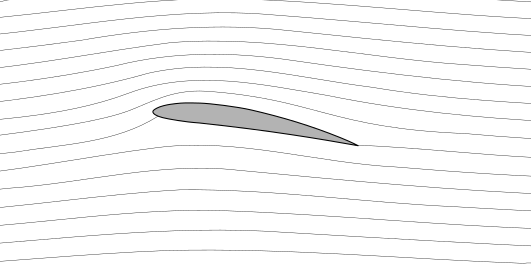
\includegraphics[width=\textwidth]{../fig/uitwendige_stroming/Vleugelprofiel_stroomlijnen}\\
		\pause
		Door het vleugelprofiel zal de stroming van richting veranderen
  	\end{frame}
%%%%%%%%%%%%%%%%%%%%%%%%%%%%%%%%%%%%%%%%%%%%%%%%%%%%%%%%%%%%%%%%%%%%%%%%%%%
  	\begin{frame}
		\frametitle{Drukverdeling}
		\vspace{0.5cm}
		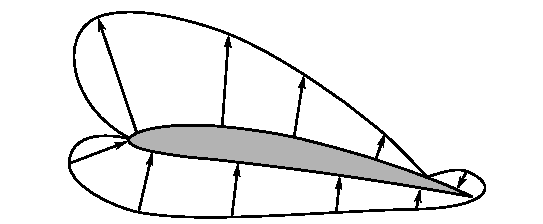
\includegraphics[width=\textwidth]{../fig/uitwendige_stroming/Vleugelprofiel_drukverdeling}
		% Demo?
  	\end{frame}
%%%%%%%%%%%%%%%%%%%%%%%%%%%%%%%%%%%%%%%%%%%%%%%%%%%%%%%%%%%%%%%%%%%%%%%%%%%
  	\begin{frame}
		\frametitle{Verloop van lift- en weerstandscoëfficiënt}
		\vspace{1cm}
		\center
		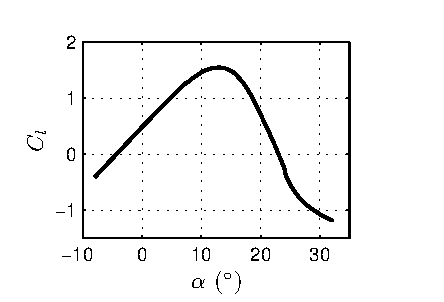
\includegraphics[width=0.49\textwidth]{../fig/uitwendige_stroming/NACA_4412_Cl}
		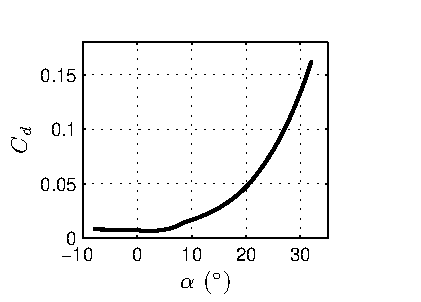
\includegraphics[width=0.49\textwidth]{../fig/uitwendige_stroming/NACA_4412_Cd}
  	\end{frame}
%%%%%%%%%%%%%%%%%%%%%%%%%%%%%%%%%%%%%%%%%%%%%%%%%%%%%%%%%%%%%%%%%%%%%%%%%%%
  	\begin{frame}
		\frametitle{Stall}
		\center
		\href{run:fig/uitwendige_stroming/Streamlines_around_an_airfoil.mp4}{
			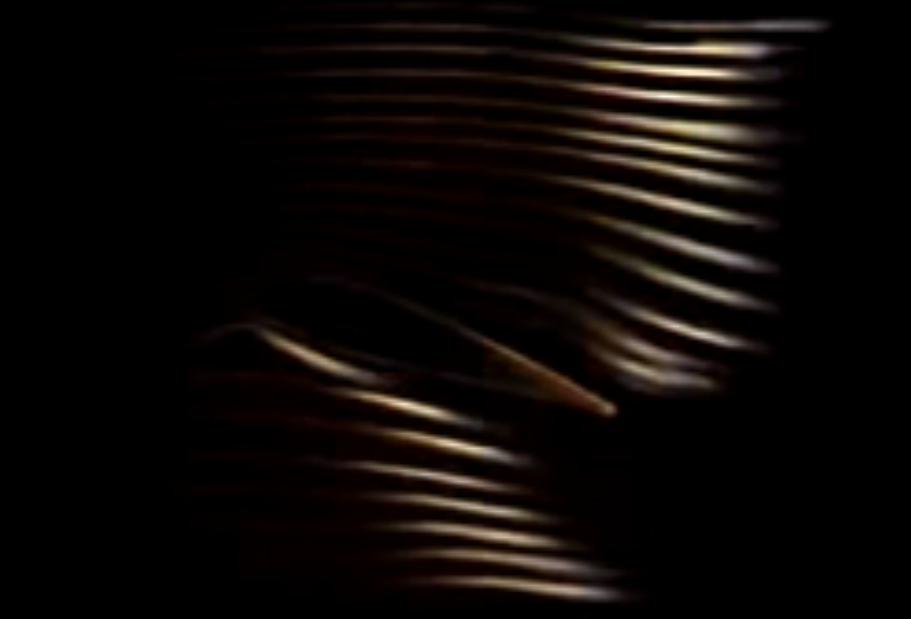
\includegraphics[width=0.8\textwidth]{../fig/uitwendige_stroming/Streamlines_around_an_airfoil.png}
		}\\
		\footnotesize{Bron: https://www.youtube.com/watch?v=6UlsArvbTeo}
  	\end{frame}
%%%%%%%%%%%%%%%%%%%%%%%%%%%%%%%%%%%%%%%%%%%%%%%%%%%%%%%%%%%%%%%%%%%%%%%%%%%
\end{document}